\documentclass[12pt]{report}
\usepackage{amsmath}
\usepackage{amssymb}
\usepackage{graphicx}
\usepackage{tikz}

\newcommand{\cosec}{\text{ cosec}}
\newcommand{\ubt}[1]{\textbf{\underline{#1}}}
\newcommand{\sps}{\\[0.2cm]}
\newcommand{\spn}[1]{\\[#1cm]}
\newcommand{\refn}[1]{\textbf{(\ref{#1})}}
\newcommand{\bt}[1]{\textbf{#1}}
\newcommand{\NCF}{Newton-Cotes Formulae}
\newcommand{\NC}{Newton-Cotes}
\newcommand{\sprime}{'}
\newcommand{\dprime}{''}
\newcommand{\tprime}{'''}
\newcommand{\dsp}{\displaystyle}
\newcommand{\NI}{\noindent}

\renewcommand{\baselinestretch}{1.5}
\renewcommand{\contentsname}{Table of Contents}

\setlength{\parindent}{1em}


\begin{document}
	
	%%%%%%%%%%%%%%%%%%%FRONT COVER%%%%%%%%%%%%%%%%%%%
	\clearpage
	\thispagestyle{empty}
	\addcontentsline{toc}{chapter}{Title Page}
	\begin{center}
		\LARGE \bt{NEWTON-COTES FORMULAE FOR NUMERICAL INTEGRATION}
	\end{center}

	\hspace{7cm}
	
	\begin{center}
		\textbf{\textit{BY}}
	\end{center}
	
	\hspace{5cm}
	
	\begin{center}
		\Large \textbf{AMAO, KAMALDEEN OLANREWAJU 
			\\
			16/56EB046}
	\end{center}
	
	\hspace{9cm}
	
	\begin{center}
		A PROJECT SUBMITTED TO THE DEPARTMENT OF MATHEMATICS, FACULTY OF PHYSICAL SCIENCES, UNIVERSITY OF ILORIN, ILORIN, KWARA STATE, NIGERIA.
	\end{center}

	\hspace{8cm} \\
	
	\begin{center}
		IN PARTIAL FULFILLMENT OF REQUIREMENTS FOR THE AWARD OF BACHELOR OF SCIENCE \textit{(B.Sc.)} DEGREE IN MATHEMATICS.
	\end{center}
	\hspace{5cm}
	\\ \\ \\
	\begin{center}
		\textbf{JUNE, 2021}
	\end{center}

	\newpage
	\pagenumbering{roman}
	\addcontentsline{toc}{chapter}{\numberline{}Certification}
	\section*{\begin{center}\textbf{\Large Certification}   \end{center}}
	This is to certify that this project was carried out by \textbf{AMAO, KAMALDEEN OLANREWAJU} of Matriculation Number  16/56EB046, for the award of Bachelor of Science B.Sc (Hons) degree in the Department of Mathematics, Faculty of Physical sciences, University of Ilorin, Ilorin, Nigeria.
	\\
	\\
	................................... \qquad \qquad\qquad\qquad\qquad\qquad...................... \\
	PROF. R.B. ADENIYI   \quad\qquad\qquad\qquad\qquad\qquad\qquad Date\\
	(SUPERVISOR)\\
	\\
	\\
	\\
	...................................... \qquad\qquad\qquad\qquad\qquad\qquad ......................\\
	PROF. K. RAUF      \quad\qquad\qquad\qquad\qquad\qquad\qquad\qquad\quad     Date\\
	(HEAD OF DEPARTMENT)\\
	\\
	\\
	\\
	..................................... \qquad\qquad\qquad\qquad\qquad\qquad .......................\\
	PROF. T. O. OLUYO  \qquad\qquad\qquad\qquad\qquad\qquad \qquad        Date\\
	(EXTERNAL EXAMINER)
	
	\newpage
	%%ACKNOLEDGEMENT%%
	\section*{\begin{center}\textbf{\Large Acknowledgments}\end{center}}
	\addcontentsline{toc}{chapter}{\numberline{}Acknowledgments} 					
	All thanks to God the Almighty, the one who is and will forever be, the one and only true God, for all He was done for me throughout the course of my academic journey in the University of Ilorin. May the name be praised forever.\\
	
	\NI I wish to express my profound gratitude to my Project Supervisor, Prof. R.B. Adeniyi for his efforts and support towards this project. May God bless you and your family Sir.\\
	
	\NI I also want to acknowledge my H.O.D, Prof. K. Rauf, and other lecturers of the department who have contributed in one way or another to my academic success: Prof. J.A Gbadeyan, Prof. T.O. Opoola, Prof. O.M. Bamigbola, Prof. M.O. Ibrahim, Prof. O.A. Taiwo, Prof. K.O. Babalola, Prof. M.S. Dada, Prof. A.S. Idowu, Doctors E.O. Titiloye, O.A. Fadipe-Joseph, Y.O, Aderinto, C.N. Ejieji, B.M. Yisa, J.U. Abubakar, K.A. Bello, G.N. Bakare, B.M. Ahmed, O.T. Olotu, I.F. Usamot, D.A. Uwaheren, O. Odetunde, T.L. Oyekunle, A.A. Yeketi, also the efforts of the non-academics staff of he department, may God reward you all and your families.\\
	
	\NI My eternal and immeasurable gratitude goes to my Dad, Mr. Amao Ganiyu and my Mom, Mrs. Amao Mulikat Taiwo, they have stood behind me solidly through all. Thank you for your words of advise, encouragement and all the efforts you have put in me to make who I am today, I will be forever be indebted to you both. God bless you abundantly.\\
	
	\NI I want to say a big thank you to all my friends who believed and still believe in me, those who helped me in one way or the other during my academic years in this school. God bless you all.\\
	
	\newpage
	
	%%%%%%%%%%%%%%%%%%%TABLE OF CONTENTS%%%%%%%%%%%%%%%%%%%
	\addcontentsline{toc}{chapter}{Table of Contents}
	\tableofcontents
	
	\newpage
	\pagenumbering{arabic}
	
	%%%%%%%%%%%%%%%%%%%CHAPTER ONE%%%%%%%%%%%%%%%%%%%
	\chapter{GENERAL INTRODUCTION}
	
	\section{INTRODUCTION}
	The general problem of numerical integration may be stated as follows. Given a set of data points $(x_0, y_0), (x_1,y_1), \cdots , (x_n,y_n)$ of a function $\displaystyle y = f(x)$ is not known explicitly, it is required to compute the value of the definite integral
	\begin{equation}
		I = \int_a^b y\text{ dx}
	\end{equation}
	As in the case of numerical differentiation, one replaces $f(x)$ by an interpolating polynomial $\phi (x)$ and obtains, an integration, integral. Thus, different integration formulae can be obtained depending upon the type of the interpolation formulae used.\sps
	\par Let the interpolation points $x_i$, be equally spaced, that is let $x_i = x_0 + ih, \; i = 0, 1, 2, \cdots , n$ and let the end points of the interval of integration be placed such that
	$$
	x_0 = a, \; \; \; \; \; x_n = b, \; \; \; \; \; h = \frac{b-a}{n} .
	$$
	Then the definite integral
	\begin{equation}
		I = \int_{a}^{b}y\text{ dx}
		\label{int1}
	\end{equation}
	is evaluated by an integration formula of the type
	\begin{equation}
		I_n = \sum_{i=0}^{n} Q_i y_i ,
		\label{ntclosed}
	\end{equation}
	where the coefficient $Q_i$ are determined completely by the abscissa $x_i$. Integration formulae of the type \refn{ntclosed} are called \textbf{Newton-Cotes Closed Integration Formulae}. They are \textbf{"closed"} since the end points $a \text{ and } b$ are the extreme abscissa in the formulae. It is easily seen that the integration formulae derived in \refn{int1} are the simplest Newton-Cotes Closed Formulae. On the other hand, formulae which do not employ the endpoints are called \bt{Newton-Cotes Open Integration Formulae}. The Newton-Cotes Formulae are an extremely useful and straightforward family of numerical integration techniques.
	
	\section{STATEMENT OF THE PROBLEM}
	In order to obtain the solution of the numerical integration using \NCF, there must be three basic steps:
	\begin{enumerate}
		\item To integrate a function $f(x)$ over some interval $[a,b]$, we divide it into $n$ equal parts such that $f_n = f(x_n)$ and $h\equiv (b-a)/n$.
		
		\item Then find the polynomials which approximate the tabulated function.
		
		\item Integrate them to approximate the Area under the curve.
	\end{enumerate}
	
	\section{AIMS AND OBJECTIVES OF THE STUDY}
	The aim of this project is to study and obtain numerical solution of integration using \NCF. The objectives were to:
	\begin{enumerate}
		\item Obtain the method which are found to give sufficient accuracy in numerical integration;
		
		\item Compare the numerical solution of the problem using the method stated in the aim with the exact value; and 
		
		\item recommend the method if it gives a sufficient accuracy for the solution of the problem.
	\end{enumerate}

	\section{SIGNIFICANCE OF STUDY}
	The method discussed in this project is extremely useful and straightforward family of numerical integration techniques. It is also used to find the fitting Polynomials which is used in Lagrange Interpolating Polynomials.
	
	\section{SCOPE OF THE STUDY}
	The scope of this project is meant to solve a numerical integration and provide a foundation knowledge for all subsequent steps in other project within the scope of work of this nature. With the knowledge of the subject, we tried to the project work explanatory by examples with concurrently understandable explanations, hereby creating a foreknowledge for people who are not familiar with the topic.
	
	\newpage
	
	%%%%%%%%%%%%%%%%%%%CHAPTER TWO%%%%%%%%%%%%%%%%%%%
	\chapter{LITERATURE REVIEW}
	
	\section{REVIEW OF RELATED LITERATURE}
	\NCF may be \bt{"closed"} if the interval $[x_1, x_2]$ is included in the fit \bt{"open"} if the points $[x_2, x_{n-1}]$ are used, or a variation of these two. If the formula uses $n$ points (closed or open), the coefficients, of terms sum to $n-1$. In 1940, Daniell obtained remainders in interpolation and quadrature formulae. Hildebrand(1967), introduced some numerical solution in numerical analysis. Whittaker and Robinson (1967), derived some formulae of integration for the \NC. Abrahmwitz and Stegun solved some problems of integration in handbook of Mathematical functions with formulae, graphs and mathematical tables. Press et al. (1992), obtained classical formulas for equally spaced abscissas.\sps
	Corbit (1996), obtained some solutions of numerical integration from Traphezoids to Root Mean Square (RMS). Ueberhuber (1997) computed some datas in numerical computations.\sps
	Fornberg(1998), calculated some weights in finite difference Formulas. Weerakoon and Fernando (2000), developed a variant of Newton's method with accelerated third-order convergence. Hasanov et al. (2002), modified Newton's method for numerical integration. Nedzhibov (2002), presented an iterative methods for solving nonlinear equations. Frontim and Sormom (2003), developed some variants of Newton's method with third order convergence.\sps
	In 2004, Ozban also developed some new variant of Newton's method. Lukic and Ralevic (2008), deduced Geometric Mean of Newton's method for simple and multiple roots.\sps
	Ababneh(2012), Solved problems on New Newton's method with third-order convergence for Solving nonlinear equations. Jain et al. (2012), established numerical methods for Scientific and engineering computation.\sps
	Jayakumar and Kalyanasundaran(2013), modified Newton's method using harmonic mean for solving nonlinear equations. More results an \NC could be seen Layakumar(2013).
	
	\section{NUMERICAL INTEGRATION}
	The general problem of numerical integration may be stated as follows. Give a set of data point $(x_0,y_0), (x_1,y_1), \cdots,(x_n,y_n)$ of a function $y=f(x)$, where $f(x)$ is not known explicitly, it is required to compute the value of definite integral
	\begin{equation}
		I = \int_{a}^{b}y \text{ dx}
		\label{eq2_2}
	\end{equation}
	As in the case of numerical differentiation, one replaces $f(x)$ by an interpolating polynomial $phi(x)$ and obtains, on integration, an approximate value of the definite integral.\sps
	Thus, different integration formulae can be obtained depending upon the type of the interpolation formulae used. Using Newton's Forward Difference Formula to derive the general formula.\sps
	Let the interval $[a,b]$ be divided into $n$ equal subintervals such that $a = x_0 < x_1 < x_2 < \cdots < x_n = b$. Clearly, $x_n = x_0 + nh$. Hence the integral becomes
	$$
		I = \int_{x_0}^{x_n} y \text{ dx}
	$$
	Approximating $y$ by Newton's Forward Difference Formula, we obtain
	$$
		I = \int_{x_0}^{x_n}\left[ y_0 + P\Delta y_0 + \frac{(P-1)}{2}\Delta^2 y_0 + \frac{P(P-1)(P-2)}{6}\Delta^3 y_0 + \cdots \right]\text{dx}
	$$
	Since $x = x_0 + Ph, \; \text{dx} = hdp$ and hence the above integral becomes
	$$
		I = h\int_{x_0}^{x_n}\left[ y_0 + P\Delta y_0 + \frac{(P-1)}{2}\Delta^2 y_0 + \frac{P(P-1)(P-2)}{6}\Delta^3 y_0 + \cdots \right]\text{dp}
	$$
	Which gives on simplification
	\begin{equation}
		\int_{x_0}^{x_n} = nh\left[ y_0 + \frac{n}{2}\Delta y_0 + \frac{n(2n-3)}{12}\Delta^2 y_0 + \frac{n(n-2)^2}{24}\Delta y_0 + \cdots \right]
		\label{eq2_3}
	\end{equation}
	From this general formula, we can obtain different integration formulae by putting $n=1,2,3, \cdots$ etc.
	
	\newpage
	
	%%%%%%%%%%%%%%%%%%%CHAPTER THREE%%%%%%%%%%%%%%%%%%%
	\chapter{THE NEWTON-COTES FORMULAE}
	
	\section{TRAPEZOIDAL RULE}
	Setting $n=1$ in the general formula in \refn{eq2_3}, all difference higher than the first will become zero and we obtain
	\begin{equation}
		\int_{x_0}^{x_1} y \text{ dx} = h(y_0 + \frac{1}{2}\Delta y_0) = h \left[ y_0 + \frac{1}{2} (y_1 - y_0) \right] = \frac{h}{2}(y_0 + y_1)
		\label{eq3_1}
	\end{equation}
	For the next interval $[x_1, x_2]$, we deduce similarly
	\begin{equation}
		\int_{x_1}^{x_2} y\text{ dx} = \frac{h}{2} (y_1+y_2)
		\label{eq3_2}
	\end{equation}
	and so on. For the last interval $[x_{n-1}, x_n]$ we have
	\begin{equation}
		\int_{x_{n-1}}^{x_n} y\text{ dx} = \frac{h}{2}(y_{n-1} + y_n)
		\label{eq3_3}
	\end{equation}
	Combining all these expressions, we obtain the
	\begin{equation}
		\int_{x_0}^{x_1} y\text{ dx} = \frac{h}{2}\left[ y_0 + 2(y_1 + y_2 + \cdots + y_{n-1}) + y_n \right]
		\label{eq3_4}
	\end{equation}
	Which is known as the \bt{Trapezoidal Rule}.\sps
	The geometrical significance of this rule is that the curve $y=f(x)$ is replaced by $n$ straight lines joining the point $(x_0,y0)$ and $(x_1,y_1), (x_1,y_1)$ and $(x_2,y_2), \cdots,(x_{n-1}, y_{n-1})$ and $(x_n, y_n)$. The area bounded by the curve $y=f(x)$, the ordinates $x=x_0$ and $x=x_n$, and the x-axis is then approximately equivalent to the sum of the areas of the $n$ trapeziums obtained. The error of the trapezoidal formula can be obtained in the following way.\sps
	Let $y=f(x)$ be continuous, well-behaved, and possess continuous derivatives in $[x_0, x_n]$. Expanding $y$ in a Taylor's series around $x=x_0$, we obtain
	\begin{eqnarray*}
		\int_{x_0}^{x_1}y\text{ dx} &=& \int_{x_1}^{x_2}\left[y_0 + (x-x_0)y_0\sprime + \frac{(x-x_0)^2}{2}y_0\dprime + \cdots \right]dx
	\end{eqnarray*}
	\begin{eqnarray}
		&=& hy_0 + \frac{h^2}{2}y_0\sprime + \frac{h^3}{6}y_0\tprime + \cdots
		\label{eq3_5}
	\end{eqnarray}
	Similarly,
	\begin{eqnarray*}
		\frac{h}{2}(y_0 + y_1) &=& \frac{h}{2}(y_0 + y_0 + hy_0\sprime + \frac{h^2}{2}y_0\dprime + \frac{h^3}{6}y_0\tprime + \cdots)
	\end{eqnarray*}
	\begin{eqnarray}
		&=&hy_0 + \frac{h^2}{2}y_0\sprime + \frac{h^3}{4}y_0\dprime + \cdots
		\label{eq3_6}
	\end{eqnarray} 
	From \refn{eq3_5} and \refn{eq3_6}, we obtain
	\begin{equation}
		\int_{x_0}^{x_n}y\text{ dx} - \frac{h}{2}(y_0 + y_1) = - \frac{1}{12}h^3y_0\dprime + \cdots,
		\label{eq3_7}
	\end{equation}
	Which is the error in the interval $[x_0, x_1]$.  Proceeding in a similar manner we obtain errors in the remaining subintervals, viz, $[x_1,x_2], [x_2,x_3], \cdots$ and $[x_{n-1}, x_n]$. We thus have
	\begin{equation}
		E = \frac{1}{12}h^3(y_0\dprime + y_1\dprime + \cdots + y_{n-1}\dprime)
		\label{eq3_8} 
	\end{equation}
	Where $E$ is the total error. Assuming that $y\dprime(\bar{x})$ is the largest value of the $n$ quantities on the right-hand of \refn{eq3_8}, we obtain
	\begin{equation}
		E = \frac{1}{12}h^3ny\dprime(\bar{x}) = - \frac{b-a}{12}h^2y\dprime(\bar{x})
		\label{eq3_9}
	\end{equation}
	Since $nh = b - a$
	
	\section{SIMPSON 1/3-RULE}
	This rule is obtained by putting $n=2$ in \refn{eq2_3}, that is by replacing the curve by $n/2$ arc of second-degree polynomials or parabolas. We have then
	$$
		\int_{x_0}^{x_2}y\text{ dx} = 2h(y_0 + \Delta y_0 + \frac{1}{6}\Delta^2 y_0) = \frac{h}{3}(y_0 + 4y_1 + y_2)
	$$
	Similarly
	$$
		\int_{x_2}^{x_4}y\text{ dx} = \frac{h}{3}(y_2 + 4y_3 + y_4)
	$$
	$$\vdots$$ $$\vdots$$
	and finally
	$$
		\int_{x_{n-2}}^{x_n}y\text{ dx} = \frac{h}{3}(y_{n-2} + 4y_{n-1} + y_n)
	$$
	summing up, we obtain
	\begin{eqnarray*}
		\int_{x_0}^{x_n} y\text{ dx} &= \frac{h}{3}\big[ y_0 + 4(y_1 + y_3 + y_5 + \cdots + y_{n-1})
	\end{eqnarray*}
	\begin{eqnarray}
		& + & 2(y_2 + y_4 + y_6 + \cdots + y_{n-2}) + y_n \big]
		\label{eq3_10}
	\end{eqnarray}
	Which is known as \bt{Simpson's $1/3$-Rule}, or simply \bt{Simpson's Rule}. It should be noted that this rule requires the division of the whole range into an even number of subintervals of width $h$.\sps
	Following the method, it can be shown that error in Simpson's rule is given by 
	\begin{eqnarray*}
		\int_{a}^{b}\text{ dx} &=& \frac{h}{3} \big[y_0 + 4\big(y_1 + y_3 + y_5 + \cdots + y_{n-1}\big) \\[0.4cm]
		&+& 2\big(y_2 + y_4 + y_6 + \cdots + y_{n-1} + y_n \big)
	\end{eqnarray*}
	\begin{eqnarray}
		 &=& \frac{b-a}{180} h^4 y^{iv}(\bar{x}), \; \; \; \; \; \; \; \; \; \; \; \; \; \; \; \; \quad
		 \label{eq3_11}
	\end{eqnarray}
	Where $y^{iv}(\bar{x})$ is the largest value of the fourth derivatives.
	
	\section{SIMPSON'S 3/8-RULE}
	Setting $n=3$ in \refn{eq2_3}, we observe that all the differences higher than the third become zero and we obtain
	\begin{eqnarray*}
		&=& 3h\big(y_0 + \frac{3}{2}\Delta y_0 + \frac{3}{4}\Delta^2 y_0 + \frac{1}{8}\Delta^3 y_0 \big) \\[0.4cm]
		&=& 3h\big[y_0 + \frac{3}{2}(y_1 -y_0) + \frac{3}{4}(y_2 - 2y_1 + y_0) + \frac{1}{8}(y_3 - 3y_2 + 3y_1 - y_0) \big] \\[0.4cm]
		&=& \frac{3h}{8}(y_0 + 3y_1 + 3y_2 + y_3)
	\end{eqnarray*}
	Similarly,
	$$
		\int_{x_3}^{x_6}y\text{ dx} = \frac{3h}{8}(y_3 + 3y_4 + 3y_5 + y_6)
	$$
	and so on. Summing up all these, we obtain
	\begin{eqnarray*}
		\int_{x_0}^{x_n}y\text{ dx} &=& \frac{3h}{8}\big[ (y_0 + 3y_1 + 3y_2 + y_3) + (y_3 + 3y_4 + 3y_5 + y_6) + \cdots \\
		&+& (y_{n-3} + 3y_{n-2} + 3y_{n-1} + y_n) \big]
	\end{eqnarray*}
	\newpage
	\begin{eqnarray*}
		&=&\frac{3h}{8}(y_0 + 3y_1 + 3y_2 + 2y_3 + 3y_4 + 3y_5 + 2y_6 + \cdots\\[-1cm]
	\end{eqnarray*}
	\begin{eqnarray}
		&+& 2y_{n-3} + 3y_{n-2} + 3y_{n-1} + y_n) \quad \quad \quad \quad \quad \quad \quad
		\label{eq3_12}
	\end{eqnarray}
	This rule, called \bt{Simpson's $3/8$-Rule}, is not so accurate as Simpson's Rule, the formula being $(3/80)h^5y^{iv}(\bar{x})$\sps
	
	\section{BOOLE'S AND WEDDLE'S RULES}
	If we wish to retain differences up to those of the fourth order, we should integrate between $x_0$ and $x_4$ and obtain \bt{Boole's Formula}
	\begin{equation}
		\int_{x_0}^{x_n}y\text{ dx} = \frac{2h}{45}\big( 7y_0 + 32y_1 + 12y_2 + 32y_3 + 7y_4\big)
		\label{eq3_13}
	\end{equation}
	The leading team in the error of this formula can shown to be 
	$$
		\frac{-8h^7}{945}y^{vi}(\bar{x})
	$$
	If, one the other hand we integrate between $x_0$ and $x_6$ retaining difference up to those of sixth order, we obtain \bt{Weddle's Rule}
	
	\begin{equation}
		\int_{x_0}^{x_6}y\text{ dx} = \frac{3h}{10}\big(y_0 + 5y_1 + y_2 + 6y_3 + y_4 + 5y_5 + y_6\big)
		\label{eq3_14} 
	\end{equation}
	the error in which is given by $-(h^7/140)y^{vi}(\bar{x})$.\sps
	These two formulae can also be generalized as in the previous cases. It should, however, be noted that the number of strips will have to be a multiple of four in the case of Boole's Rule and a multiple of six for Weddle's Rule.
	
	\section{USE OF CUBIC SPLINES}
	If $S(x)$ is the \bt{Cubic Spline} in the interval $(x_{i-1}, x_{i})$, then we have
	
	\begin{eqnarray*}
		I &=& \int_{x_0}^{x_n}y\text{ dx} \approx \sum_{i=1}^{n}\int_{{x_{i-1}}}^{x_i}S(x)\text{ dx}\sps
		&=& \sum_{i=x_{i-1}}^{n}\int_{x_{i-1}}^{x_i}\left\{\frac{1}{6h}\left[(x_i - x)^3M_{i-1} + (x-x_{i-1})^3M_i\right]\right. \sps
		&+&\left.\frac{1}{h}(x_i - x)\left[y_{i-1} - \frac{h^2}{6}M_{i-1}\right] +\frac{1}{h}(x-x_{i-1})\left(y_i - \frac{h^2}{6}M_i \right)\right\}\text{dx}
	\end{eqnarray*}
	Using
	\begin{eqnarray*}
		S_i(x) &=& \frac{1}{h_i}\left[\frac{(x_i - x)^3}{6}M_{i-1} + \frac{(x-x_{i-1})^3}{6}M_i + \left(y_{i-1} - \frac{h_i^2}{6}M_{i-1}\right)(x_i-x)\right. \sps
		&+& \left.\left(y_i - \frac{h_i^2}{6}M_i(x-x_{i-1})\right) \right]
	\end{eqnarray*}
	On carrying out the integration and simplifying, we obtain
	\begin{equation}
		I = \sum_{i=1}^{n}\left[\frac{h}{2}(y_{i-1} + y_i) - \frac{h^3}{24}(M_{i-1} + M_i)\right]
		\label{eq3_15}
	\end{equation}
	Where $M_i$, the \bt{Spline Second-derivatives}, are calculated from recurrence relation
	$$
		M_{i-1} + 4M_i + M_{i+1} = \frac{6}{h^2}(y_{i-1} - 2y_i + y_{i+1}), \; i=1,2,\cdots,n-1
	$$
	
	\section{ROMBERG INTEGRATION}
	This method can often be used to improve the approximate results obtained by the finite-difference methods. It application to the numerical evaluation of definite integrals, for example in the use of Trapezoidal Rule, can be described, as follows.\sps
	We consider the integral
	$$
		I = \int_{a}^{b}y\text{ dx}
	$$
	and evaluate it by the Trapezoidal Rule \refn{eq3_3} with two different subintervals of widths $h_1$ and $h_2$ to obtain the approximate values $I_1$ and $I_2$, respectively. Then \refn{eq3_9} gives errors $E_1$ and $E_2$ as
	\begin{equation}
		E_1 = -\frac{1}{12}(b-a)h^2, \; y\dprime(\bar{x})
		\label{eq3_16}
	\end{equation}
	and
	\begin{equation}
		E_2 = -\frac{1}{12}(b-a)h^2, \; y\dprime(\bar{\bar{x}})
		\label{eq3_17}
	\end{equation}
	Since the term $y\dprime(\bar{\bar{x}})$ in \refn{eq3_17} is also the largest value of $y\dprime$, it is reasonable to assume that the quantities $y\dprime(\bar{x})$ and $y\dprime(\bar{\bar{x}})$ are very nearly the same. We therefore have
	$$
		\frac{E_1}{E_2} = \frac{h_1^2}{h_2^2}
	$$
	and hence
	$$
	\frac{E_2}{E_2 -E_1} = \frac{h_2^2}{h_2^2 - h_1^2}
	$$
	Since $E_2 - E_1 = I_2 - I_1$, this gives
	\begin{equation}
		E_2 = \frac{h_2^2}{h_2^2 - h_1^2}(I_2 - I_1)
		\label{eq3_18}
	\end{equation}
	We therefore obtain a new approximation $I_3$ defined by
	\begin{equation}
		I_3 = I_2 - E_2 = \frac{I_1h_2^2 - I_2h_1^2}{h_2^2 - h_1^2}
		\label{eq3_19}
	\end{equation}
	Which, in general, would be closer to the actual value provided that the errors decrease monotonically and are the same sign.\sps
	If we now set
	$$
		h_2 = \frac{1}{2}h_1 = \frac{1}{2}h
	$$
	eqn \refn{eq3_19} can be written in the more convenient form
	\begin{equation}
		I\left(h,\frac{1}{2}h\right) = \frac{1}{3}\left[4I\left(\frac{1}{2}h\right)- I\left(h\right)\right]
		\label{eq3_20}
	\end{equation}
	Where $I(h) = I_1, \; I(\frac{1}{2}h) = I_2$ and $I(h,\frac{1}{2}h) = I_3$\sps
	with this notation, the following table can be formed
	$$\begin{array}{cccc}
		I(h) & & &\\
		& I(h,\frac{1}{2}h) & & \\
		I(\frac{1}{2}h) & & I(h, \frac{1}{2}h, \frac{1}{4}h)& \\
		& I(\frac{1}{2}h, \frac{1}{4}h) & & I(h, \frac{1}{2}h, \frac{1}{4}h,\frac{1}{8}h)\\
		I(\frac{1}{4}h) & & I(\frac{1}{2}h, \frac{1}{4}h,\frac{1}{8}h) & \\
		& I(\frac{1}{4}h,\frac{1}{8}h)& &\\
		I(\frac{1}{8}h) & & & \\
	\end{array}$$
	The computations can be stopped when two successive values are sufficiently close to each other. This method, due to L.F. Richardson, is called the deferred approach to the limit and Systematic tabulation of this is called \bt{Romberg Integration}.
	
	\section{NEWTON-COTES INTEGRATION FORMULAE}
	Let the interpolation points, $x_i$, be equally spaced, that is let $x_i = x_0 + ih$, $i=0,1,2,\cdots,n$, and let the endpoints of the interval of integration be placed such that
	$$
		x_0 = a, \quad x_n = b, \quad h = \frac{b-a}{n}
	$$
	The definite integral
	\begin{equation}
		I = \int_{a}^{b}y\text{ dx}
		\label{eq3_21}
	\end{equation}
	is evaluated by an integration formula of the type
	\begin{equation}
		I_n = \sum_{i=0}^{n} c_iy_i
		\label{eq3_22}
	\end{equation}
	Where the coefficients $c_i$ are determined completely by the abscissa $x_i$. Integration Formulae of the type \refn{eq3_22} are called \bt{Newton-Cotes Closed Integration Formulae}.\sps
	They are \bt{"closed"} since the endpoints $a$ and $b$ are extreme abscissa in the formulae. It is easily seen that the integration formulae derived eqns \refn{eq3_18} - \refn{eq3_21} are simplest Newton-Cotes Closed Formulae.\sps
	On the other hand, formulae which do not employ the endpoints are called \bt{Newton-Cotes, Open Integration Formulae}.\sps
	We give below the five simplest Newton-Cotes Open Integration Formulae
	\begin{eqnarray}
		\text{(i)}  \int_{x_0}^{x_2}y\text{ dx} &=& 2hy_1 + \frac{h^3}{3}y\dprime(\bar{x}), (x_0 \leq \bar{x} < x_2)\\[1cm]
		\text{(ii)}  \int_{x_0}^{x_3}y\text{ dx} &=& \frac{3h}{2}(y_1 + y_2)+ \frac{3h^3}{4}y\dprime(\bar{x}), (x_0 < \bar{x} < x_3)\\[1cm]
		\text{(iii)}  \int_{x_0}^{x_4}y\text{ dx} &=& \frac{4h}{3}(2y_1 - y_2 + 2y_3)+\frac{14}{45}h^5y^{iv}(\bar{x}),\nonumber\\
		& &(x_0 \leq \bar{x} < x_4)
	\end{eqnarray}
	\newpage
	\begin{eqnarray}
		\text{(iv)}  \int_{x_0}^{x_5}y\text{ dx} &=& \frac{5h}{24}(11y_1 + y_2 + y_3 + 11y_4)\nonumber\\
		&+&\frac{95}{144}h^5y^{iv}(\bar{x}), (x_0 < \bar{x} < x_5) \\[1cm]
		\text{(v)}  \int_{x_0}^{x_6}y\text{ dx} &=& \frac{6h}{20}(11y_1-14y_2+26y_3-14y_4+11y_5)\nonumber\\
		&+& \frac{41}{140}h^7y^{vi}(\bar{x}),(x_0 < \bar{x} < x_6)
	\end{eqnarray}
	A convenient method for determining the coefficients in the Newton-Cotes Formulae is the method of \bt{Undetermined Coefficients}.
	
	\section{PRINCIPLE OF NEWTON-COTES INTEGRATION}
	This subsection only cover the Newton-Cotes closed formulas.\sps
	The interval of integration $[a,b]$ is partitioned by the points.
	$$
		\left\{a,a + \frac{b-a}{n}, a+2 \cdot \frac{b-a}{n}, \cdots, b\right\}
	$$
	We estimate the integral of $f(x)$ on this interval by using the Lagrange Interpolating Polynomial through the following points.
	$$
		\left\{\left(a,f(a)\right), \left(a + \frac{b-a}{n}, f\left(a + \frac{b-a}{n}\right)\right), \cdots,\left(b, f(b)\right)\right\}
	$$
	The formula for the integral of this Lagrange Polynomial simplifies to a linear combination of the values of $f(x)$ at the points
	$$
		\left\{x_i = a + i \cdot \frac{b-a}{n} \;\arrowvert \; i=0,1,2,3,\cdots,n \right\}
	$$
	
	\section{ERROR ANALYSIS OF NEWTON-COTES}
	One would expect that the error would grow smaller as we use larger $n$ in the Newton-Cotes method. It turns out that this not correct. The reason is that using equally spaced points, the Lagrange interpolating Polynomial may give a very bad approximation of the function away from the interpolating points. It can be so bad that the integrals of these polynomials do not converge to the integral of the function $f(x)$ as $n \rightarrow \infty$.\sps
	The classic example is the following function over the interval $[-4,4]$
	$$
		f(x) = \frac{1}{1 + x^2}
	$$
	
	%%%%%%%%%%%%%%%%%%%CHAPTER FOUR%%%%%%%%%%%%%%%%%%%
	\chapter{COMPUTATIONAL PROBLEMS}
	In this chapter, three problems was solved by Closed Newton-Cotes Formulae and the results obtained  were compared with the exact solution.\\
	
	\section{NUMERICAL EXAMPLES}
	\ubt{Example 4.1}\\
	Consider the integral:
	$$
		\int_{\frac{\pi}{4}}^{\frac{\pi}{2}} \frac{\sin x}{x} \text{ dx},\qquad h = \frac{\pi}{24}
	$$
	\newpage
	Solving for the exact value\spn{0.6}
	(1)$\dsp\int_{\frac{\pi}{4}}^{\frac{\pi}{2}} \frac{\sin x}{x} \text{ dx},\quad h = \frac{\pi}{24}$\spn{0.5}
	By trigonometry identity\\
	$\dsp \sin x = 2 \sin(\frac{x}{2})\cos(\frac{x}{2})$\\
	\\Let $\dsp I = \int \frac{\sin x}{x} \text{ dx}$\spn{0.6}
	$\dsp I = \int \frac{2\sin(\frac{x}{2})\cos(\frac{x}{2})\text{ dx}}{x}$\spn{0.7}
	$\dsp I = \int \frac{\sin(\frac{x}{2})\cos(\frac{x}{2})}{\frac{x}{2}}\text{ dx}$\spn{0.7}
	Put $\dsp \sin \frac{x}{2} = t \implies \frac{x}{2} = \sin^{-1}(t)$\\
	
	$\dsp \implies \frac{\text{dt}}{\text{dx}} = \frac{1}{2}\cos(\frac{x}{2})$\spn{-.2}
	
	$\dsp \implies \cos(\frac{x}{2})\text{dx} = 2\text{dt} $\sps
	
	Therefore,\\
	$$
		I = 2 \int\frac{t\text{ dt}}{\sin^{-1}(t)}
	$$
	$$
		2\int t\text{ cosec}(t)\text{ dt}
	$$
	Integrating by parts\\
	\begin{eqnarray*}
		I &=& 2 \left[\cosec^{-1}t \cdot \frac{t^2}{2} - \int\frac{-1}{t\sqrt{t^2-1}}\cdot \frac{t^2}{2}\text{ dt}\right]\spn{0.5}
		&=& 2\left[\frac{t^2\cosec^{-1}(t)}{2} + \frac{1}{2}\int\frac{t}{\sqrt{t^2-1}}\text{ dt}\right]
	\end{eqnarray*}

	\NI Let $u = t^2 - 1$ du$ = 2t$dt $\frac{\text{du}}{2} = t\text{ dt}$\\
	\begin{eqnarray*}
		&=& 2\left[\frac{t^2\cosec^{-1}(t)}{2} + \frac{1}{2}\int\frac{1}{\sqrt{2}}\frac{\text{du}}{2}\right]\quad\spn{0.5}
		&=& t^2\cosec^{-1}(t) + \frac{1}{2} \frac{u^{\frac{1}{2}}}{-\frac{1}{2} + 1} + C\quad\spn{0.5}
		&=& t^2\cosec^{-1}(t) + \sqrt{u}\qquad\qquad\spn{0.5}
		&=& \frac{\sin^{2}(\frac{x}{2})}{\sin^{-1}(\frac{x}{2})} + \sqrt{\sin^2 \frac{x}{2}-1} + C \spn{0.5}
		I&=& \frac{2\sin^{2}(\frac{x}{2})}{x} + \sqrt{\sin^2 \left(\frac{x}{2}\right)-1} + C
	\end{eqnarray*}
	\\So, for $\dsp \int_{\frac{\pi}{4}}^{\frac{\pi}{2}}\frac{\sin x}{x} \text{ dx}$\\
	we have
	\begin{eqnarray*}
		&=& \left[\frac{2\sin^2(\frac{x}{2})}{x} + \sqrt{\sin^2(\frac{x}{2})-1}\right]_{\frac{\pi}{4}}^{\frac{\pi}{2}}\qquad\qquad\qquad\qquad\qquad\qquad\qquad\qquad\qquad\qquad\spn{0.5} 
		&=& \left[\frac{2\sin^2(\frac{\pi}{4})}{\frac{\pi}{2}} + \sqrt{\sin^2(\frac{\pi}{4})-1} \quad \right] - \left[\frac{2\sin^2(\frac{\pi}{8})}{\frac{\pi}{4}} + \sqrt{\sin^2(\frac{\pi}{8})-1} \quad \right]\spn{0.5}
		&=& \left[\frac{2(\frac{1}{2})}{\frac{\pi}{2}} + \sqrt{\frac{1}{2}-1} \quad \right] - \left[\frac{2(0.146)}{\frac{\pi}{4}} + \sqrt{(0.146)-1} \quad \right]\spn{0.3}	
		&=& 0.611786\spn{-0.3}
		&\approxeq& \mathbf{0.6118}	
	\end{eqnarray*}
	
	\newpage
	$$
		f(x) = \frac{\sin x}{x}, \qquad	 \text{ Let }  h \frac{\pi}{24}\qquad\qquad\qquad\qquad\qquad\qquad\qquad\qquad\qquad
	$$\spn{-0.9}
	\begin{center}
		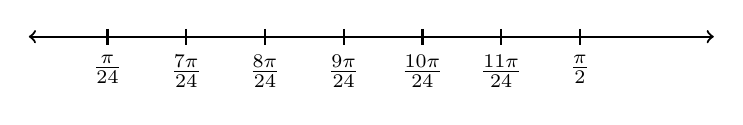
\begin{tikzpicture}
			\draw[thick, <->] (-1,0) -- (7.7,0);
			\foreach \x / \y in {0/$\frac{\pi}{24}$,1/$\frac{7\pi}{24}$,2/$\frac{8\pi}{24}$,3/$\frac{9\pi}{24}$,4/$\frac{10\pi}{24}$,5/$\frac{11\pi}{24}$,6/$\frac{\pi}{2}$}
				\draw[thick] (\x,0.1) -- (\x,-0.1) node[below] {\y}; 
		\end{tikzpicture}
	\end{center}
	\begin{eqnarray*}
		x_0 = \frac{\pi}{24} \implies f(\frac{\pi}{24}) = \frac{\sin \frac{\pi}{24}}{\frac{\pi}{24}} = \frac{0.7071}{45} = 0.0157\qquad\qquad \spn{0.5}
		x_1 = \frac{7\pi}{24} \implies f(\frac{7\pi}{24}) = \frac{\sin(\frac{7\pi}{24})}{\frac{7\pi}{24}} = \frac{0.7934}{52.5} = 0.0151\qquad\spn{0.5}
		x_2 = \frac{8\pi}{24} \implies f(\frac{8\pi}{24}) = \frac{\sin(\frac{8\pi}{24})}{\frac{8\pi}{24}} = \frac{0.8660}{60} = 0.0144\qquad\spn{0.5}
		x_3 = \frac{9\pi}{24} \implies f(\frac{9\pi}{24}) = \frac{\sin(\frac{9\pi}{24})}{\frac{9\pi}{24}} = \frac{0.9239}{67.5} = 0.0137\qquad\spn{0.5}
		x_4 = \frac{10\pi}{24} \implies f(\frac{10\pi}{24}) = \frac{\sin(\frac{10\pi}{24})}{\frac{10\pi}{24}} = \frac{0.9659}{75} = 0.0129\;\;\spn{0.5}
		x_5 = \frac{11\pi}{24} \implies f(\frac{11\pi}{24}) = \frac{\sin(\frac{11\pi}{24})}{\frac{11\pi}{24}} = \frac{0.9914}{82.5} = 0.0120\;\;\spn{0.5}
		x_6 = \frac{\pi}{2} \implies f(\frac{\pi}{2}) = \frac{\sin(\frac{\pi}{2})}{\frac{\pi}{2}} = \frac{1}{90} = 0.0
		11\qquad\qquad\quad\;\;\spn{0.5}
	\end{eqnarray*}
	\ubt{Using Trapezoidal}
	\begin{equation*}
		T_n = \frac{h}{2}\left[f(x_0) + 2f(x_1) + 2f(x_{n-1}) + \cdots + f(x_n)\right]\qquad\qquad\qquad
	\end{equation*}
	\begin{eqnarray*}
		T_6 &=& \frac{7.5}{2}\left[0.0157 + 2(0.0151) + 2(0.014) + 2(0.0137) + 2(0.0129) + 2(0.0120) + 0.0111\right]\spn{0.5}
		&=& \frac{7.5}{2}\left[0.0157 + 0.0302 + 0.0288 + 0.0274 + 0.0258 + 0.024 + 0.0111\right]\spn{0.5}
		&=&3.75[0.163]\spn{0.5}
		&=&0.61125\spn{0.5}
		&\approxeq& 0.6113
	\end{eqnarray*}
	\\
	\NI\ubt{Using Simpson 1/3-Rule}
	$$
		S_n = \frac{h}{3}\left[f(x_0) + 4f(x_1) + 2f(x_2) + 4f(x_{n-1}) + \cdots f(x_n)\right]\qquad\qquad\qquad\qquad\qquad
	$$
	\begin{eqnarray*}
		S_6 &=&\frac{7.5}{3}\left[0.0157 + 4(0.0151) + 2(0.0144) + 4(0.0137) + 2(0.0129) + 4(0.0120) + 0.0111\right]\spn{0.5}
		&=&\frac{7.5}{3}[0.0157 + 0.0604 + 0.0288 + 0.0548 + 0.0258 + 0.048 + 0.011]\spn{0.5}
		&=& 2.5[0.2446]\spn{0.5}
		&\approx& 0.6115
	\end{eqnarray*}
	\newpage
	\NI\ubt{Using Simpson 3/8-Rule}
	$$
		S_n = \frac{3h}{8}\left[f(x_0) + 3f(x_1) + 3f(x_2)+ 2f(x_3) + 3f(x_{n-1})  + f(x_n)\right]
	$$
	\begin{eqnarray*}
		S_6 &=&\frac{3(7.5)}{8}\left[0.0157 + 3(0.0151) + 3(0.0144) + 2(0.0137) + 3(0.0129) + 3(0.0120) + 0.0111\right]\spn{0.5}
		&=&2.8125[0.0157 + 0.0453 + 0.0432 + 0.0274 + 0.0387 + 0.011]\spn{0.5}
		&=& 2.8125[0.2174]\spn{0.1}
		&=& 0.61144375\spn{0.1}
		&\approx& 0.6114
	\end{eqnarray*}
	\\
	\NI\ubt{Using Boole's Rule}
	$$
	B_n = \frac{2h}{45}\left[7f(x_0) + 32f(x_1) + 12f(x_2)+ 32f(x_3) + 7f(x_4)\right]\qquad\qquad\qquad\qquad\qquad
	$$
	\begin{eqnarray*}
		B_6 &=&\frac{2(7.5)}{45}\left[7(0.0157) + 32(0.0151) + 12(0.0144) + 32(0.0137) + 12(0.0129) + 32(0.0120) + 7(0.0111)\right]\spn{0.5}
		&=&0.33[0.1099 + 0.4832 + 0.1728+ 0.4384 + 0.1548 + 0.384 + 0.0777]\spn{0.5}
		&=& 0.33[1.8208]\spn{0.1}
		&=& 0.600864\spn{0.1}
		&\approx& 0.6009
	\end{eqnarray*}
	\newpage
	\ubt{Example 4.2}\\
	$$
		\int_{0}^{\pi} \frac{\text{dx}}{x + \cos x}, \quad h=\frac{\pi}{4}, \quad h=\frac{\pi}{8}\qquad\qquad\qquad\qquad\qquad\qquad\qquad
	$$
	\ubt{Solution}\\
	$$
		f(x) = \frac{1}{x + \cos x}\qquad\qquad\qquad\qquad\qquad\qquad\qquad\qquad\qquad\qquad\qquad\qquad\qquad\qquad\qquad
	$$\spn{-0.6}
	\begin{center}
		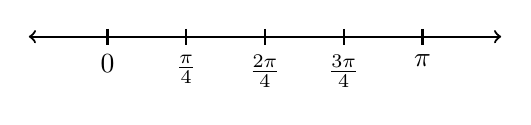
\begin{tikzpicture}
			\draw[thick, <->] (0,0) -- (6,0);
			\foreach \x / \y in {1/$0$,2/$\frac{\pi}{4}$,3/$\frac{2\pi}{4}$,4/$\frac{3\pi}{4}$,5/$\pi$}
			\draw[thick] (\x,0.1) -- (\x,-0.1) node[below] {\y}; 
		\end{tikzpicture}
	\end{center}
	\begin{eqnarray*}
		x_0 &=& 0 \implies f(0) = \frac{1}{0 + \cos 0} = \frac{1}{1} = 1\spn{0.3}
		x_1 &=& \frac{\pi}{4} \implies f\left(\frac{\pi}{4}\right) = \frac{1}{\frac{\pi}{4} + \cos \left(\frac{\pi}{4}\right)} = \frac{1}{45 + 0.7071} = \frac{1}{45.7071} = 0.0219\spn{0.5}
		x_2 &=& \frac{2\pi}{4} \implies f\left(\frac{2\pi}{4}\right) = \frac{1}{\frac{2\pi}{4} + \cos \left(\frac{2\pi}{4}\right)} = \frac{1}{90 + 0} = 0.0111\spn{0.5}
		x_3 &=& \frac{3\pi}{4} \implies f\left(3\frac{\pi}{4}\right) = \frac{1}{\frac{3\pi}{4} + \cos \left(\frac{3\pi}{4}\right)} = \frac{1}{135 + (-0.7071)} = \frac{1}{134.2929} = 0.0074\spn{0.5}
		x_4 &=& \pi \implies f\left(\pi\right) = \frac{1}{\pi + \cos \left(\pi\right)} = \frac{1}{180 + (-1)} = \frac{1}{179} = 0.0056\spn{0.5}
	\end{eqnarray*}
	\ubt{Using Trapezoidal}
	\begin{equation*}
		T_n = \frac{h}{2}\left[f(x_0) + 2f(x_1) + 2f(x_{n-1}) + \cdots + f(x_n)\right]\qquad\qquad\qquad
	\end{equation*}
	\begin{eqnarray*}
		T_4 &=& \frac{45}{2}\left[1 + 2(0.0219) + 2(0.0111) + 2(0.074) _ 0.0056\right]\qquad\qquad\qquad\quad\spn{0.5}
		&=& 22.5\left[1 + 0.0438 + 0.0222 + 0.0148 + 0.0056\right]\spn{0.5}
		&=&22.5[1.2196]\spn{0.5}
		&=&27.441
	\end{eqnarray*}
	\ubt{Using Simpson 1/3-Rule}
	\begin{equation*}
		S_n = \frac{h}{3}\left[f(x_0) + 4f(x_1) + 2f(x_2) + 4f(x_{n-1}) + \cdots f(x_n)\right]\qquad\qquad\qquad\qquad\qquad
	\end{equation*}
	\begin{eqnarray*}
		S_4 &=& \frac{45}{3}\left[1 + 4(0.219) + 2(0.0111) + 4(0.0074) + 0.0056\right]\qquad\qquad\qquad\quad\spn{0.5}
		&=& 15\left[1 + + 0.876 + 0.0222 + 0.0296 + 0.0056\right]\spn{0.5}
		&=&15[1.9574]\spn{0.5}
		&=&29.361
	\end{eqnarray*}
	\newpage
	\NI\ubt{Using Simpson 3/8-Rule}
	$$
		S_n = \frac{3h}{8}\left[f(x_0) + 3f(x_1) + 3f(x_2)+ 2f(x_3) + 3f(x_{n-1})  + f(x_n)\right]
	$$
	\begin{eqnarray*}
		S_4 &=&\frac{3(45)}{8}\left[1 + 3(0.0219) + 3(0.0111) + 2(0.0074) + 0.0056\right]\spn{0.5}
		&=&16.875[1 + 0.0657 + 0.0333 + 0.0148 + 0.0056]\spn{0.5}
		&=&16.875[1.1194]\spn{0.1}
		&=& 18.889875\spn{0.1}
		&\approx& 18.89
	\end{eqnarray*}
	\NI\ubt{Using Boole's Rule}
	$$
		B_n = \frac{2h}{45}\left[7f(x_0) + 32f(x_1) + 12f(x_2)+ 32f(x_3) + 7f(x_4)\right]\qquad\qquad\qquad\qquad\qquad
	$$
	\begin{eqnarray*}
		B_4 &=&\frac{2(45)}{45}\left[7(1) + 32(0.0219) + 12(0.0111) + 32(0.0074) + 7(0.0056)\right]\spn{0.5}
		&=&2[7 + 0.7008 + 0.1332 + 0.2368 + 0.0392]\spn{0.5}
		&=& 2[8.11]\spn{0.1}
		&=& 16.22\spn{0.1}
	\end{eqnarray*}
	\ubt{2nd Solution}\\
	$$
		\int_{0}^{\pi} \frac{\text{dx}}{x + \cos x}, \quad h=\frac{\pi}{8}\qquad\qquad\qquad\qquad\qquad\qquad\qquad\qquad\qquad\qquad
	$$
	$$
		f(x) = \frac{1}{x + \cos x}\qquad\qquad\qquad\qquad
	$$\\
	
	\begin{center}
		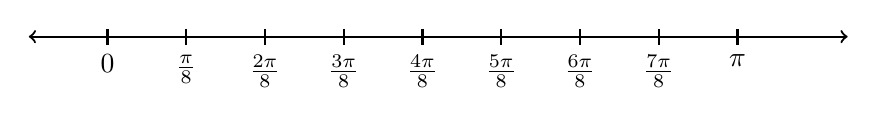
\begin{tikzpicture}
			\draw[thick, <->] (-1,0) -- (9.4,0);
			\foreach \x / \y in {0/$0$,1/$\frac{\pi}{8}$,2/$\frac{2\pi}{8}$,3/$\frac{3\pi}{8}$,4/$\frac{4\pi}{8}$,5/$\frac{5\pi}{8}$,6/$\frac{6\pi}{8}$,7/$\frac{7\pi}{8}$,8/$\pi$}
			\draw[thick] (\x,0.1) -- (\x,-0.1) node[below] {\y}; 
		\end{tikzpicture}
	\end{center}
	
	\begin{eqnarray*}
		x_0 &=& 0 \implies f(0) = \frac{1}{0 + \cos 0} = \frac{1}{1} = 1\spn{0.3}
		x_1 &=& \frac{\pi}{8} \implies f\left(\frac{\pi}{8}\right) = \frac{1}{\frac{\pi}{8} + \cos \left(\frac{\pi}{8}\right)} = \frac{1}{22.5 + 0.9239} = \frac{1}{23.4239} = 0.0427\spn{0.5}
		x_2 &=& \frac{2\pi}{8} \implies f\left(\frac{2\pi}{8}\right) = \frac{1}{\frac{2\pi}{8} + \cos \left(\frac{2\pi}{8}\right)} = \frac{1}{45 + \cos 45} = 0.0219\spn{0.5}
		x_3 &=& \frac{3\pi}{8} \implies f\left(\frac{3\pi}{8}\right) = \frac{1}{\frac{3\pi}{8} + \cos \left(\frac{3\pi}{8}\right)} = \frac{1}{135 + (-0.7071)} = \frac{1}{134.2929} = 0.0074\spn{0.5}
		x_4 &=& \frac{4\pi}{8} \implies f\left(\frac{4\pi}{8}\right) = \frac{1}{\frac{4\pi}{8} + \cos \left(\frac{4\pi}{8}\right)} = \frac{1}{90 + \cos 90} = 0.0111\spn{0.5}
		x_5 &=& \frac{5\pi}{8} \implies f\left(\frac{5\pi}{8}\right) = \frac{1}{\frac{5\pi}{8} + \cos \left(\frac{5\pi}{8}\right)} = \frac{1}{112.5 + (-0.3827)} = \frac{1}{112.1173} =  0.0089\spn{0.5}
		x_6 &=& \frac{6\pi}{8} \implies f\left(\frac{6\pi}{8}\right) = \frac{1}{\frac{6\pi}{8} + \cos \left(\frac{6\pi}{8}\right)} = \frac{1}{135 + \cos 135} = 0.0074\spn{0.5}
	\end{eqnarray*}
	\newpage
	\begin{eqnarray*}
		x_7 &=& \frac{7\pi}{8} \implies f\left(\frac{7\pi}{8}\right) = \frac{1}{\frac{7\pi}{8} + \cos \left(\frac{7\pi}{8}\right)} = \frac{1}{157.5 + (-0.9239)} = \frac{1}{156.5761} =  0.0064\spn{0.5}
		x_8 &=& \pi \implies f\left(\pi\right) = \frac{1}{\pi + \cos \left(\pi\right)} = \frac{1}{180 + (-1)} = 0.0056\spn{0.5}
	\end{eqnarray*}
	\ubt{Using Trapezoidal}
	\begin{equation*}
		T_n = \frac{h}{2}\left[f(x_0) + 2f(x_1) + 2f(x_{n-1}) + \cdots + f(x_n)\right]\qquad\qquad\qquad
	\end{equation*}
	\begin{eqnarray*}
		T_8 &=& \frac{22.5}{2}\left[1 + 2(0.0427) + 2(0.0219) + 2(0.0147) + 2(0.0111) + 2(0.0089) \right.\\ 
		&+&\left. 2(0.0074) + 2(0.0064) + 0.0056\right]\spn{0.5}
		&=& 11.25\left[1 + 0.0854 + 0.0438 + 0.0294 + 0.0222 + 0.0178 + 0.0148 \right.\\ 
		&+&\left. 0.0128 + 0.0056 \right]\spn{0.2}
		&=& 11.25[1.2318]\spn{0.1}
		&=&13.85775\spn{0.1}
		&\approx& 13.86
	\end{eqnarray*}
		\ubt{Using Simpson 1/3-Rule}
	\begin{equation*}
		S_n = \frac{h}{3}\left[f(x_0) + 4f(x_1) + 2f(x_2) + 4f(x_{n-1}) + \cdots f(x_n)\right]\qquad\qquad\qquad\qquad\qquad
	\end{equation*}
	\begin{eqnarray*}
		S_8 &=& \frac{22.5}{3}\left[1 + 4(0.0427) + 2(0.0219) + 4(0.0147) + 2(0.0111) + 4(0.0089) \right.\\ 
		&+&\left. 2(0.0074) + 4(0.0064) + 0.0056\right]\spn{0.5}
		&=& 7.5\left[1 + 0.1708 + 0.0438 + 0.0588 + 0.0222 + 0.0356 + 0.0148 \right.\\ 
		&+&\left. 0.0256 + 0.0056 \right]\spn{0.2}
		&=& 7.5[1.3772]\spn{0.1}
		&=&10.329\spn{0.1}
	\end{eqnarray*}

	\NI\ubt{Using Simpson 3/8-Rule}
	$$
		S_n = \frac{3h}{8}\left[f(x_0) + 3f(x_1) + 3f(x_2)+ 2f(x_3) + 3f(x_{n-1})  + f(x_n)\right]
	$$
	\begin{eqnarray*}
		S_8 &=& \frac{3(22.5)}{8}\left[1 + 3(0.0427) + 3(0.0219) + 2(0.0147) + 3(0.0111) + 3(0.0089) \right.\\ 
		&+&\left. 2(0.0074) + 3(0.0064) + 0.0056\right]\spn{0.5}
		&=& 8.4375\left[1 + 0.1281 + 0.0657 + 0.0294 + 0.0333 + 0.0267 + 0.0148 \right.\\ 
		&+&\left. 0.0192 + 0.0056 \right]\spn{0.2}
		&=& 8.4375[1.3228]\spn{0.1}
		&=&11.161125\spn{0.1}
		&\approx& 11.16
	\end{eqnarray*}
	\newpage
	\NI\ubt{Using Boole's Rule}
	$$
		B_n = \frac{2h}{45}\left[7f(x_0) + 32f(x_1) + 12f(x_2)+ 32f(x_3) + 7f(x_4)\right]\qquad\qquad\qquad\qquad\qquad
	$$
	\begin{eqnarray*}
		B_8 &=& \frac{2(22.5)}{45}\left[7(1) + 32(0.0427) + 12(0.0219) + 32(0.0147) + 12(0.0111) + 32(0.0089) \right.\\ 
		&+&\left. 12(0.0074) + 32(0.0064) + 7(0.0056)\right]\spn{0.5}
		&=& \frac{45}{45}\left[7 + 1.3664 + 0.2628 + 0.4704 + 0.1332 + 0.2848 + 0.0888 \right.\\ 
		&+&\left. 0.2048 + 0.00392 \right]\spn{0.2}
		&=&9.8504\spn{0.1}
		&\approx& 9.850
	\end{eqnarray*}
	\newpage
	\ubt{Example 4.3}\\
	$$
	\int_{0}^{\pi} \frac{\text{dx}}{1 + x^2}, \quad h=\frac{\pi}{4}, \qquad\qquad\qquad\qquad\qquad\qquad\qquad\qquad\qquad\qquad
	$$\sps
	\ubt{Solution}\sps
	$\dsp
		\int_{0}^{\pi} \frac{1}{1 + x^2}\text{d}x\sps
		\text{Let } x = \tan u\sps
		\text{d}x = \sec^2u\text{d}u\sps
		\int_{0}^{\pi} \frac{1}{1 + \tan^2 u} \cdot \sec^2 u \text{d}u\sps
		\int_{0}^{\pi} \frac{1}{\sec^2 u} \cdot \sec^2 u \text{d}u\sps
		\int_{0}^{\pi}\text{d}u\sps
		\implies u\Big|_0^\pi \sps
		= \tan^{-1}(x)\Big|_0^\pi\sps
		= \tan^{-1}(\pi)\sps
		= 1.26262725\spn{0.5}
	$\sps
	$\dsp
		f(x) = \frac{\text{d}x}{1 + x^2}, \qquad \text{let }h=\frac{\pi}{4}\spn{0.5}
	$
	\newpage
	$\dsp
		f(x) = \frac{\text{d}x}{1 + x^2}\sps
	$\sps
	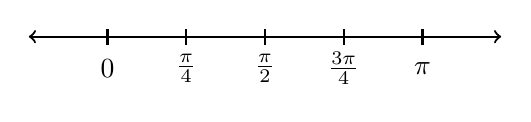
\begin{tikzpicture}
		\draw[thick,<->] (-1,0)--(5,0);
		\foreach \x in {0,1,...,4}
			\draw[thick] (\x,-0.1) -- (\x,0.1);
		
		\node at (0,-0.4){$0$};
		\node at (1,-0.4){$\frac{\pi}{4}$};
		\node at (2,-0.4){$\frac{\pi}{2}$};
		\node at (3,-0.4){$\frac{3\pi}{4}$};
		\node at (4,-0.4){$\pi$};
	\end{tikzpicture}
	\begin{eqnarray}
		x_0 &=& 0 \implies f(0) = \frac{1}{1+(2)^2} = \frac{1}{1} = 1\notag\sps
		%%%
		x_1 &=& \frac{\pi}{4} \implies f(\frac{\pi}{4}) = \frac{1}{1+\left(\frac{\pi}{4}\right)^2} = \frac{1}{1.61685} = 0.061848\notag\sps
		%%%
		x_2 &=& \frac{\pi}{2} \implies f(\frac{\pi}{2}) = \frac{1}{1 + \left(\frac{\pi}{2}\right)^2} = \frac{1}{3.46740} = 0.28868 \notag\sps
		%%%
		x_3 &=& \frac{3\pi}{4} \implies f(\frac{3\pi}{4}) = \frac{1}{1 + \left(\frac{3\pi}{4}\right)^2} = \frac{1}{6.55165} = 0.15263\notag\sps
		%%%
		x_4 &=& \pi \implies f(\pi) = \frac{1}{1+(\pi)^2} = \frac{1}{4.14169} = 0.24145\notag
		%%%
	\end{eqnarray}
	\ubt{Using Trapezoidal}
	\begin{eqnarray}
		T_n &=& \frac{h}{2}\left[f(x_0) + 2f(x_1) + 2f(x_{n-1}) + \cdots + f(x_n))\right]\notag\spn{0.1}
		%%%
		T_4 &=& \frac{\pi}{8}\left[f(x_0)+2f(x_1) + 2f(x_2)+2f(x_3) + f(x_4)\right]\notag\spn{0.1}
		&=& \frac{\pi}{8}\left[1+2(0.61848) + 2(0.28868)+2(0.15263)+0.24145\right]\notag\spn{0.1}
		&=&0.39269(1+1.36368+0.57736+0.30526+0.24145)\notag\spn{0.1}
		&=&0.39269(3.48775)\notag\spn{0.1}
		&=&1.36960\notag
	\end{eqnarray}
	\ubt{Using Simpson 1/3 Rule}
	\begin{eqnarray}
		S_n &=& \frac{h}{3}\left[f(x_0)+4f(x_1)+2f(x_2)+4f(x_{n-1}) + \cdots + f(x_n)\right]\notag\spn{0.1}
		%%%
		S_4 &=& \frac{h}{3}(f(x_0) + 4f(x_1) + 2f(x_2) + 4f(x_3) + f(x_4))\notag\spn{0.1}
		%%%
		S_4 &=& \frac{\pi}{12}(1 + 4(0.61848) + 2(0.28868) + 4(0.15263)+0.24145)\notag\spn{0.1}
		%%%
		&=& 0.26179(1+2.47392 + 0.57736 + 0.61052 + 0.24145)\notag\spn{0.1}
		%%%
		&=& 0.26179(4.90325)\notag\spn{0.1}
		%%%
		&=& 1.28362\notag 
	\end{eqnarray}
	\ubt{Using Simpson 3/8 Rule}
	\begin{eqnarray}
		S_n &=& \frac{3h}{8}\left[f(x_0)+3f(x_1) + 3f(x_2) + 2f(x_3) + 3f(x_{n-1}) + f(x_n)\right]\notag\spn{0.1}
		%%%
		S_4 &=& \frac{3h}{8}(f(x_0) + 3f(x_1) + 3f(x_2) + 2f(x_3) + f(x_4)) \notag\spn{0.1}
		%%%
		&=&\frac{3\pi}{32}(1+3(0.61848)+3(0.28868)+2(0.15263)+0.24145)\notag\spn{0.1}
		%%%
		&=&0.29452(1+1.85544+0.86604 +0.30526+0.24145)\notag\spn{0.1}
		%%%
		&=&0.29452(4.26819)\notag\spn{0.1}
		%%%
		&=& 1.25706\notag
	\end{eqnarray}

	\ubt{Using Boole's Rule}
	\begin{eqnarray}
		B_n &=&  \frac{2h}{45}(7f(x_0) + 32f(x_1)+12f(x_2)+32f(x_3)7f(x_4))\notag\spn{0.1}
		%%%
		B_4 &=&\frac{2h}{45}(7f(x_0) + 32f(x_1)+12f(x_2)+32f(x_3)7f(x_4))\notag\spn{0.1}
		%%%
		B_4 &=& \frac{\pi}{90}(7(1)+32(0.61848)+12(0.28868)+32(0.15263)+7(0.24145))\notag\spn{0.1}
		%%%
		&=& 0.03490(7+19.79136+3.46416+4.88416+1.69015)\notag\spn{0.1}
		%%%
		&=&0.03490(36.82983)\notag\spn{0.1}
		%%%
		&=& 1.28536\notag
	\end{eqnarray}

	\begin{table}[!thb]
		\begin{center}
			\begin{tabular}{|l|c|c|}
				\hline
				\multicolumn{2}{|c|}{Methods}& Error\\ \hline
				Exact & 0.6118& \\ \hline
				Trapezoidal & 0.6113 & 0.0005 \\ \hline
				Simpson 1/3-rule & 0.6115 & 0.0003 \\ \hline
				Simpson 3/8-rule & 0.6114 & 0.0004 \\ \hline
				Boole's rule & 0.6009 & 0.0109\\ \hline
			\end{tabular}
		\end{center}
		\caption{(Result for Example 1)}
		\label{tb:4_1}
	\end{table}

	\begin{table}[!hbt]
		\begin{center}
			\begin{tabular}{|l|c|c|}
				\hline
				\multicolumn{2}{|c|}{Methods}& Error\\ \hline
				Exact & 29.889& \\ \hline
				Trapezoidal & 27.441 & 2.448 \\ \hline
				Simpson 1/3-rule & 29.361 & 0.528 \\ \hline
				Simpson 3/8-rule & 18.890 & 10.999 \\ \hline
				Boole's rule & 16.220 & 13.669\\ \hline
			\end{tabular}
		\end{center}
		\caption{(Result for Example 2, $\dsp h=\frac{\pi}{4}$)}
		\label{tb:4_2}
	\end{table}
	\begin{table}[!hbt]
		\begin{center}
			\begin{tabular}{|l|c|c|}
				\hline
				\multicolumn{2}{|c|}{Methods}& Error\\ \hline
				Exact & 29.889 &  \\ \hline
				Trapezoidal & 13.860 & 16.029 \\ \hline
				Simpson 1/3-rule & 10.329 & 19.56 \\ \hline
				Simpson 3/8-rule & 11.160 & 18.729 \\ \hline
				Boole's rule & 9.850 & 20.039\\ \hline
			\end{tabular}
		\end{center}
		\caption{(Result for Example 2, $\dsp h=\frac{\pi}{8}$)}
		\label{tb:4_3}
	\end{table}
	\begin{table}[h]
		\begin{center}
			\begin{tabular}{|l|c|c|}
				\hline
				\multicolumn{2}{|c|}{Methods}& Error\\ \hline
				Exact & 29.889 &  \\ \hline
				Trapezoidal & 13.860 & 0.10698 \\ \hline
				Simpson 1/3-rule & 10.329 & 0.021 \\ \hline
				Simpson 3/8-rule & 11.160 & 0.0056 \\ \hline
				Boole's rule & 9.850 & 0.02274\\ \hline
			\end{tabular}
		\end{center}
		\caption{(Result for Example 3, $\dsp h=\frac{\pi}{4}$)}
		\label{tb:4_4}
	\end{table}
	\newpage
	$\left.\right.$\spn{0.8}
	\section{DISCUSSION OF RESULTS}
	In Table \refn{tb:4_1},it shown that Simpson 1/3-rule is the most accurate of the Closed \NCF and its also shows that Boole's rule is the least accurate of the Closed \NCF.\\
	
	\NI Table \refn{tb:4_2} also shows that Simpson 1/3-rule is the most accurate, while Boole's rule is also the least accurate among the Closed \NCF.
	
	
	
	%%%%%%%%%%%%%%%%%%%CHAPTER FIVE%%%%%%%%%%%%%%%%%%%
	\chapter{SUMMARY, CONCLUSION AND RECOMMENDATION}
	\section{SUMMARY}
	%The solution of closed Newton-Cotes Formulae for Numerical Integration has been presented in this study.
	
	%\NI The history of Newton and Newton-Cotes solution of Numerical Integration were also discussed in this study.
	
	%\NI Furthermore, Newton-Cotes Formulae was derived using Trapezoidal, Simpson 1/3-rule, Simpson 3/8-rule and Boole's rule which where all considered as closed Newton-Cotes Formulae.
	
	The numerical solution of definite integration by some Newton-Cotes formulae has been presented. For this projects, the Trapezoidal, Simpson's $\dsp \frac{1}{3}$, Simpson's $\dsp \frac{3}{8}$ and Boole quadrature formulae were adopted. The derivative of these formulae was also documented. The numerical solutions were applied to three selected problems and the numerical results were compared with the exact solution. These results confirm the accuracy of the schemes.
	
	
	
	\section{CONCLUSION}
	In the course of this study, it was numerical integration examples considered that Simpson 1/3-rule is the most accurate of the closed Newton-Cotes Formulae.
	
	\section{RECOMMENDATION}
	Based on what we have considered in this study, it was shown closed Newton-Cotes Formulae for Numerical Integration produced near accurate value to the exact.\\
	
	\NI It is recommended that a formulae be done so that it value could be compare with the most accurate of the closed Newton-Cotes Formulae.
	



\end{document}